%%%%%%%%%%%%%%%%%%%%%%%%%%%%%%%%
%                              %
% Luther Michaels              % 
% ECE 351-52                   %
% Lab 8                        %
% October 28, 2021             %
% Fourier Series Approximation % 
%             of a Square Wave %
%                       Prelab %
%                              %
%%%%%%%%%%%%%%%%%%%%%%%%%%%%%%%%

%%%%%%%%%%%%%%%%%%%%%%%%%%%%%%%%%%%%%%%%%%%
%%% DOCUMENT PREAMBLE %%%
\documentclass[12pt]{report}
\usepackage[english]{babel}
\usepackage{url}
\usepackage[utf8x]{inputenc}
\usepackage{amsmath}
\usepackage{graphicx}
\graphicspath{{images/}}
\usepackage{parskip}
\usepackage{fancyhdr}
\usepackage{vmargin}
\usepackage{listings}
\usepackage{hyperref}
\usepackage{xcolor}

\definecolor{codegreen}{rgb}{0,0.6,0}
\definecolor{codegray}{rgb}{0.5,0.5,0.5}
\definecolor{codeblue}{rgb}{0,0,0.95}
\definecolor{backcolour}{rgb}{0.95,0.95,0.92}

\lstdefinestyle{mystyle}{
	backgroundcolor=\color{backcolour},   
	commentstyle=\color{codegreen},
	keywordstyle=\color{codeblue},
	numberstyle=\tiny\color{codegray},
	stringstyle=\color{codegreen},
	basicstyle=\ttfamily\footnotesize,
	breakatwhitespace=false,         
	breaklines=true,                 
	captionpos=b,                    
	keepspaces=true,                 
	numbers=left,                    
	numbersep=5pt,                  
	showspaces=false,                
	showstringspaces=false,
	showtabs=false,                  
	tabsize=2
}

\lstset{style=mystyle}

\setmarginsrb{3 cm}{2.5 cm}{3 cm}{2.5 cm}{1 cm}{1.5 cm}{1 cm}{1.5 cm}

\title{8}	% Title						
\author{Luther Michaels}	% Author		
\date{October 28, 2021}   % Date

\makeatletter
\let\thetitle\@title
\let\theauthor\@author
\let\thedate\@date
\makeatother

\pagestyle{fancy}
\fancyhf{}
\rhead{\theauthor}
\lhead{\thetitle}
\cfoot{\thepage}
%%%%%%%%%%%%%%%%%%%%%%%%%%%%%%%%%%%%%%%%%%%%

\begin{document}
	
%%%%%%%%%%%%%%%%%%%%%%%%%%%%%%%%%%%%%%%%%%%%%%%%%%%%%%%%%%%%%%%%%%%%%%%%%%%%%%%%%%
%%% TITLE PAGE %%%
\begin{titlepage}
	\centering
	\vspace*{0.5 cm}
		
	\begin{center}    
		\textsc{\Large   ECE 351 - Section \#52}\\[2.0 cm]	
	\end{center}  
	\textsc{\Large Fourier Series Approximation \\ of a Square Wave  }\\[0.5 cm]
	\rule{\linewidth}{0.2 mm} \\[0.4 cm]
	{ \huge \bfseries \thetitle}\\
	\rule{\linewidth}{0.2 mm} \\[1.5 cm]
	\begin{minipage}{0.4\textwidth}
		\begin{flushleft} \large
		\end{flushleft}
	\end{minipage}~
	\begin{minipage}{0.4\textwidth}
		\begin{flushright} \large
			\emph{Submitted By:} \\
			Luther Michaels \break
			
			\emph{Submission Date:} \\
			October 28, 2021
		\end{flushright}
	\end{minipage}\\[2 cm]
\end{titlepage}
	
%%%%%%%%%%%%%%%%%%%%%%%%%%%%%%%%%%%%%%%%%%%%%%%%%%%%%%%%%%%%%%%%%%%%%%%%%%%%%%%%%%
%%% TABLE OF CONTENTS %%%

\tableofcontents
\pagebreak

%%%%%%%%%%%%%%%%%%%%%%%%%%%%%%%%%%%%%%%%%%%%%%%%%%%%%%%%%%%%%%%%%%%%%%%%%%%%%%%%%%
%%% LAB REPORT %%%
\renewcommand{\thesection}{\arabic{section}}
\section{Introduction}

The principle focus of this lab is on approximating periodic signals with Fourier Series. The goal is to implement the derived Fourier Series of a given square wave in Python and verify that its behavior approximates that of the original signal. The initial coefficient terms of the series will be analyzed alongside plots varying the number of included terms. \\ 

An important concept for periodic signals is that of symmetry. Functions with symmetry can be classified as either even, where they are mapped identically around the y-axis, or odd, where the corresponding magnitudes about the y-axis are equal, but their signs are inverted. An even series would then be best represented solely by its cosine term with coefficient $ a_k $, while an odd would only require its sine term with $ b_k $. This procedure utilizes a derivation of the Fourier Series $ x(t) $ and its sinusoidal term coefficients $ a_k $ and $ b_k $ found in the prelab assignment. All output and plots can be produced through Python implementation written within the Spyder software. \\

\section{Equations}

\begin{align}
	x(t) &= \frac{1}{2}a_0 + \sum_{k=1}^{\infty}a_kcos(kw_0t) + b_ksin(kw_0t) \\
	&= \sum_{k=1}^{\infty}\frac{2}{k\pi}[1 - cos(k\pi)]sin(\frac{2\pi kt}{T}) \nonumber
\end{align}
\begin{align}
	a_k &= \frac{2}{T}\int_{0}^{T}x(t)cos(kw_0t)dt \\
	&= 0 \nonumber
\end{align}
\begin{align}
	b_k &= \frac{2}{T}\int_{0}^{T}x(t)sin(kw_0t)dt \\
	&= \frac{2}{k\pi}[1 - cos(k\pi)]
\end{align}
\begin{equation}
	w_0 = \frac{2\pi}{T}
\end{equation}

\section{Methodology}

The first task of Part 1 requested that the Fourier Series approximation $ x(t) $ of the square wave shown in the lab manual be implemented in Python utilizing its derived terms $ a_k $ and $ b_k $. The software would then be used to print its initial coefficient terms $ a_0 $, $ a_1 $, $ b_1 $, $ b_2 $, and $ b_3 $. After identifying $ x(t) $ as an odd function, the value of $ a_k $ described by Equation 2 was immediately input as zero for all values of $ k $. The derivation of $ b_k $ first found in the prelab is shown below, from which the solution of Equation 3 could be given a function in Python. The initial terms of $ a_k $ were printed as zero, while the values of $ b_k $ were returned after passing the requested values of $ k $ to the function. 
\begin{align*}
	b_k &= \frac{2}{T}\int_{0}^{T}x(t)sin(kw_0t)dt \\
	&= \frac{2}{T}\int_{0}^{T}(1)sin(kw_0t)dt \\
	&= \frac{4}{T}\int_{0}^{\frac{T}{2}}(1)sin(kw_0t)dt \\
	&= \frac{4}{T}\frac{-1}{kw_0}cos(kw_0t)|_0^{\frac{T}{2}} \\
	&= \frac{4}{T}\frac{-1}{kw_0}[\frac{cos(kw_0T)}{2} - cos(0)] \\
	&= \frac{4}{T}\frac{-T}{2\pi k}[\frac{cos(\frac{2\pi kT}{T})}{2} - 1] \\
	&= \frac{2}{k\pi}[1 - cos(k\pi)]
\end{align*}

The general form of Equation 1 could be reduced utilizing the evaluation of $ b_k $ given by Equation 4 and the prior realization that $ a_0 $ must be zero for an odd series. The final Fourier Series $ x(t) $ found below was written as its own function in Python, implementing the summation with a loop that iterated through all values of $ k $ up to argument $ N $.
\begin{align*}
	x(t) &= \frac{1}{2}a_0 + \sum_{k=1}^{\infty}a_kcos(kw_0t) + b_ksin(kw_0t) \\
	&= \frac{1}{2}(0) + \sum_{k=1}^{\infty}(0)(cos(\frac{2\pi kt}{T}) + \frac{2}{k\pi}[1 - cos(k\pi)]sin(\frac{2\pi kt}{T}) \\
	&= \sum_{k=1}^{\infty}\frac{2}{k\pi}[1 - cos(k\pi)]sin(\frac{2\pi kt}{T})
\end{align*}

Task 2 of Part 1 asked that the Fourier Series approximations of the square wave be plotted for varying upper summation bounds prescribed by $ N = \{1,3,15,50,150,1500\} $. The value of variable $ T $ included in Equation 5 for the fundamental frequency was globally assigned a value of eight. The step size supplying good resolution was assigned $ 1 \times 10^{-5} $, and the time interval of $ [0,20s] $ was set using numpy.arange(). Two plots each containing three subplots were formatted and labeled using the commands of matplotlib.pyplot. Each $ y $ input for the plots was given the $ x(t) $ function passed the next value of $ N $ requested. \\

Github Link: \url{https://github.com/Luther-Michaels} \\

\section{Results}

Using Python to evaluate, the values of the initial coefficient terms were found as follows: $ a_0 = a_1 = b_2 = 0 $, $ b_1 = 1.27 $, $ b_3 = 0.42 $. The printed results of $ a_0 $, $ a_1 $, $ b_1 $, $ b_2 $, and $ b_3 $ are provided in the appendix. Looking at the values of $ a_k $, these results make sense given the odd symmetry of the function. Because the series can be represented solely by the sine term, the cosine term coefficient should clearly be zero to remove it entirely. The value of $ b_2 $ being zero also matches expectations given Equation 4, as the even multiple of $ \pi $ will drive the inner cosine to be $ 1 $ such that the factor subtracts to zero. Since the cosine will reduce to $ -1 $ for even $ k $, the other two values of $ b_k $ should be equivalent to $\frac{4}{k\pi} $, which proves to be the case when evaluated. \\

The three plots of the Fourier Series approximation $ x(t) $ for $ N = 1 $, $ 3 $, and $ 15 $ are shown as separate subplots in the graph below. The step size clearly provides good resolution, and the time interval has been properly set to span from $ 0 $ to $ 20s $ as requested. Given that $ N $ indicates the number of terms being included in the approximation, it makes sense that the plots with higher $ N $ values are better representations of the square wave. As the first subplot is only a single term, it clearly displays the dominant sine present in the equation. By the third subplot, it is clear that the series moves between $ -1 $ and $ 1 $ on the y-axis as in the original wave. Since $ T $ is eight, we anticipate that one period of the signal will be completed at time $ t = 8 $, which is shown to be accurate according to the plots. The greatest variation from the square wave occurs where the sharp edges of the original shape should be. \\

\begin{center}
	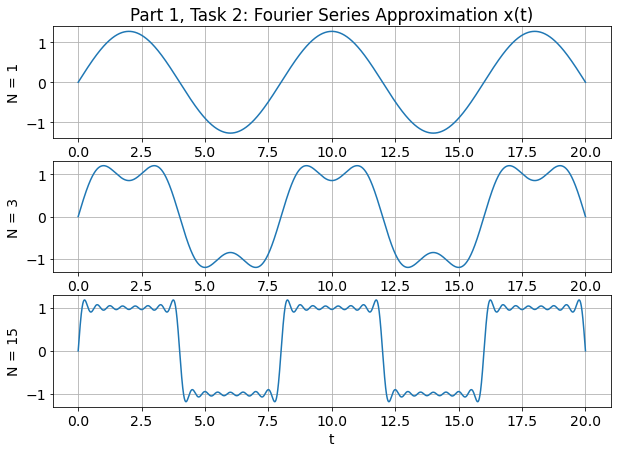
\includegraphics[scale = 0.48]{Lab 8 - Plots/Part1-Task2(1).png}\\[1.0 cm]
\end{center}

The following set of plots shows the Fourier Series approximations for $ N = 50 $, $ 150 $, and $ 1500 $. The x-axis and y-axes of the three subplots properly correspond to those in the prior graph, displaying their shapes with good resolution. One period is represented across eight seconds as the value of $ T $ would warrant. Like the other plots, the higher values of $ N $ lead to more accurate approximations of the wave. The last subplot is the best representation of the signal as we expect. Again, the approximation struggles to capture the sharp edges without rising beyond the amplitude. \\

\begin{center}
	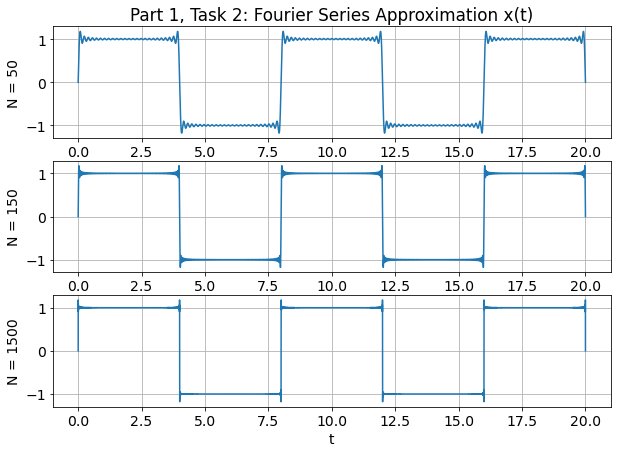
\includegraphics[scale = 0.48]{Lab 8 - Plots/Part1-Task2(2).png}\\[1.0 cm]
\end{center}

\section{Error Analysis}

The only part of this procedure that was initially a challenge was deriving the Fourier Series in the prelab assignment. I initially made the problem much more difficult be forgetting about the symmetry. I did not set $ a_k $ to zero; I also did not double a single integral to find $ b_k $. I only came to the proper solution during the lab session when the results were presented and the concept of symmetry discussed. \\

\section{Questions}

1. The function $ x(t) $ is odd. This is because all $ x(t) = -x(-t) $. Put another way, for every set of corresponding points about the y-axis, their magnitudes are equal but with opposite signs. The fact that the series $ x(t) $ is represented by the sine shape is also an indication that it must be odd given that sine is an odd function. \\

2. Based on your results from Task 1, I would expect the values of $ a_2 $, $ a_3 $, $ ... $ to all be zero. As discussed in the prior section, the series $ x(t) $ has odd symmetry and consequently only utilizes its sine terms. This is why throughout this entire procedure $ a_k $ was given to be zero. There should be no cosine portion. A derivation using Equation 2 would ultimately reveal the inclusion of a $ sin(k\pi) $ factor which is zero for all values of $ k $. \\ 

3. The approximation of the square wave improves as the value of $ N $ increases, as shown in the plots for Task 2. The Fourier Series struggles to approximate the sharp edges present in the original square wave. This means that any time there should be a perfect right angle, the approximation cannot match it and ends up moving beyond the regular pulse shape. \\

4. As the value of $ N $ increases, the number of terms included in the Fourier Series summation is increasing. While Equation 1 shows the upper summation bound of $ x(t) $to be infinity, the value is actually represented in the Python implementation with the variable $ N $. The increasing values of $ N $ correspond to an increasing range for the summation index $ k $ to operate within. In this case, the value of $ N $ does not directly indicate the number of terms affecting the result, since only odd values of $ k $ contribute to the series. \\

5. The lab tasks, expectations, and deliverables were all presented clearly.

\section{Conclusion}

This lab gave us practice working with Fourier Series to approximate periodic signals and allowed us to verify the results of our derivations. It provided clear examples illustrating the effects of the various terms that comprise the general Fourier Series equation. It also gave us a feel for how many terms may be required for a satisfactory approximation of a wave. \\

If this lab were to be repeated, I would make the prelab assignment part of the lab procedure itself. The actual lab portion is extremely short and simple compared to others and including the derivation would allow for students to seek help more readily. Trying to solve for $ a_k $ and $ b_k $ is already rather difficult alone since most of the examples in our textbook utilize the complex method to solve for Fourier Series approximations. In this lab, I learned that considering the symmetry of a signal is one of the best places to start an analysis. This will surely aid in any future problems involving Fourier Series approximations and is once again a reminder to always try to reason through and simplify a problem before diving into the mathematics. \\ 

\newpage
\appendix
\section*{Appendix - Print Output}

Part 1, Task 1:
\begin{center}
	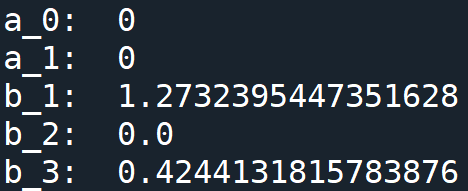
\includegraphics[scale = 0.8]{Lab 8 - Print Output/Part1-Task1.png}\\[1.0 cm]
\end{center}

\newpage
\begin{thebibliography}{111}
	
	\bibitem{S}
	Sullivan, Dennis M. (2018) {\it  Signals and Systems for Electrical Engineers I}. Nevada: CreateSpace Independent Publishing Platform.
	
\end{thebibliography}
\end{document}

% Lab Report based on template created by Roza Aceska.